\documentclass{article}
% \usepackage{showframe}
\usepackage{siunitx}
\usepackage{booktabs}
\usepackage{graphicx}
\usepackage{amsmath}
\usepackage{mathtools}
\usepackage{minted}
\usepackage{tabularx}
\usepackage{url}
% \usepackage{subfig}
\usemintedstyle{xcode}

% \usepackage{fullpage}

\frenchspacing
% \setlength{\parindent}{0ex}
% \setlength{\parskip}{3 ex plus 2 ex minus 1 ex}

\title{Homework 5}
\author{Josh Bradt}
\date{February 22, 2016}

\begin{document}

\maketitle

\section{Performance estimates}

    For the operation over one vector,
    \begin{minted}[gobble=8]{C}
        s0 = 0;
        for (i=0; i<n; i++) {
            s0 += w[i] * v[i];       // n(2r+2c)
        }
        for (i=0; i<n; i++) {
            w[i] = w[i] - s0 * v[i]; // n(2r+w+2c)
        }
    \end{minted}
    the total time estimate is
    \begin{equation}
        t_1 \approx kn(5m+4c)
    \end{equation}
    for $k$ vectors with memory access time $m$ and operation time $c$.

    For the operation over four vectors at once,
    \begin{minted}[gobble=8]{C}
        s0 = 0, s1 = 0, s2 = 0, s3 = 0;
        for (i=0; i<n; i++) {
            wi = w[i];          // n(r)
            s0 += wi * v0[i];   // n(r+2c)
            s1 += wi * v1[i];   // n(r+2c)
            s2 += wi * v2[i];   // n(r+2c)
            s3 += wi * v3[i];   // n(r+2c)
        }
        for (i=0; i<n; i++) {
            w[i] = w[i] - s0 * v0[i] - s1 * v1[i]
                        - s2 * v2[i] - s3 * v3[i];  // n(5r+8c+w)
        }
    \end{minted}
    the total time estimate is
    \begin{equation}
        t_4 \approx \frac{k}{4}n(11m+16c) = kn(2.75m+4c)
    \end{equation}
    for $k$ vectors, assuming $k$ is divisible by 4.

    The ratio between these two times is
    \begin{equation}
        \frac{t_1}{t_4} = \frac{5m+4c}{2.75m+4c} \approx \frac{5}{2.75} \approx 1.82
    \end{equation}
    assuming $m \gg c$. This is a good improvement for relatively little work.

\section{Performance measurements}

    I compiled the provided code on my Mac Mini (Intel Core i7-3615QM) with four different compilers: Intel ICC version 16.0.1, GCC version 5.2.0, Clang\footnote{Binary downloaded from \url{llvm.org/releases}} version 3.7.0, and Apple Clang\footnote{The default build that comes with OS X 10.11} version 7.0.2. The flags used for each are shown in Table~\ref{tab:flags}. The results of running the code built by each compiler are listed in Table~\ref{tab:results} and plotted in Figure~\ref{fig:results}.

    \begin{table}[tb]
        \centering
        \begin{tabularx}{\textwidth}{lX}
            \toprule
            Compiler & Flags \\
            \midrule
            Intel & \texttt{-std=c99 -O3 -DHAVE\_ICC  -xHOST -qopt-report} \\
            GCC & \texttt{-std=c99 -O3 -fivopts -flax-vector-conversions -funsafe-math-optimizations -msse4.2 -fopt-info-vec-missed} \\
            Clang / Apple Clang & \texttt{-std=c99 -O3 -flax-vector-conversions -funsafe-math-optimizations -march=native -Rpass=loop-vectorize -Rpass-missed=loop-vectorize} \\
            \bottomrule
        \end{tabularx}
        \caption{Compiler flags used for each measurement.}
        \label{tab:flags}
    \end{table}

    As expected, the version which used four separate operations (``sep op'') was slower than the one that calculated everything in one function. In all cases except for the Intel compiler, the difference is near a factor of 2, as shown above. GCC and the Intel compiler both produced slower code when the function to call was located in a separate translation unit (``sep file'' and ``$w+1$''), but neither Clang compiler showed this effect. There was no appreciable difference between the ``sep file'' and ``$w+1$'' cases, which isn't surprising since they are essentially the same code called with different pointers. (Though I'm frankly not sure what the purpose of this ``$w+1$'' case was.) Finally, using the \texttt{restrict} keyword only had a noticeable effect for the Intel compiler, where it more than doubled the performance.

    \begin{figure}
        \centering
        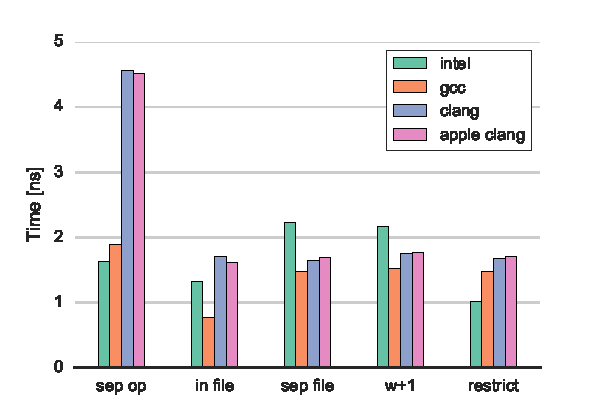
\includegraphics{barplot.pdf}
        \caption{A plot of the timing results for each compiler.}
        \label{fig:results}
    \end{figure}

    \begin{table}
        \centering
        \begin{tabular}{cccccc}
            \toprule
            Compiler    & Sep. op. & In file & Sep. file & $w+1$ & Restrict \\
            \midrule
            Intel       & 1.63     & 1.32    & 2.23      & 2.17  & 1.02     \\
            GCC         & 1.89     & 0.77    & 1.47      & 1.52  & 1.47     \\
            Clang       & 4.56     & 1.70    & 1.64      & 1.75  & 1.67     \\
            Apple Clang & 4.52     & 1.62    & 1.69      & 1.77  & 1.70     \\
            \bottomrule
        \end{tabular}
        \caption{Timing results for each compiler. All times are given in nanoseconds.}
        \label{tab:results}
    \end{table}

    Each of these compilers can produce a report on how well it vectorized the code. A basic summary of these reports is shown in Table~\ref{tab:vec}. The Intel compiler did the best job of vectorizing the loops, while GCC did the worst job. It's surprising that GCC claims to have not vectorized any of the loops since it had the best performance for many of the cases.

    \begin{table}
        \centering
        \begin{tabular}{ccccc}
            \toprule
            Function & Intel & GCC & Clang & Apple Clang \\
            \midrule
            \texttt{morth1} & All & None & Second & Second \\
            \texttt{sorth1} & First & None & Second & Second \\
            \texttt{morthf} & First & None & Second & Second \\
            \texttt{morthfr} & All & None & Second & Second \\
            \bottomrule
        \end{tabular}
        \caption{Summary of vectorization reports from each compiler. Each function consists of two loops: one to calculate the dot product and a second to subtract the results from $w$. A result of ``All'' means that both of these loops were vectorized, while ``First'', ``Second'', and ``None'' mean that only the respective loops (or neither) were vectorized.}
        \label{tab:vec}
    \end{table}

\end{document}
